\chapter{Results}\label{chapter:results}

\section{Generation Process}

Comparison of the two algorithms
Comparison of what happens with different settings for probability -> sufficiently large number of tangrams generated no visible difference on the first 6 tangrams

\section{Interestingness Measures}

Results of different measures

\subsection{User testing}

In addition to the interface described in the begin of chapter \ref{chapter:design} evaluation interface 
\begin{figure}
\centering
    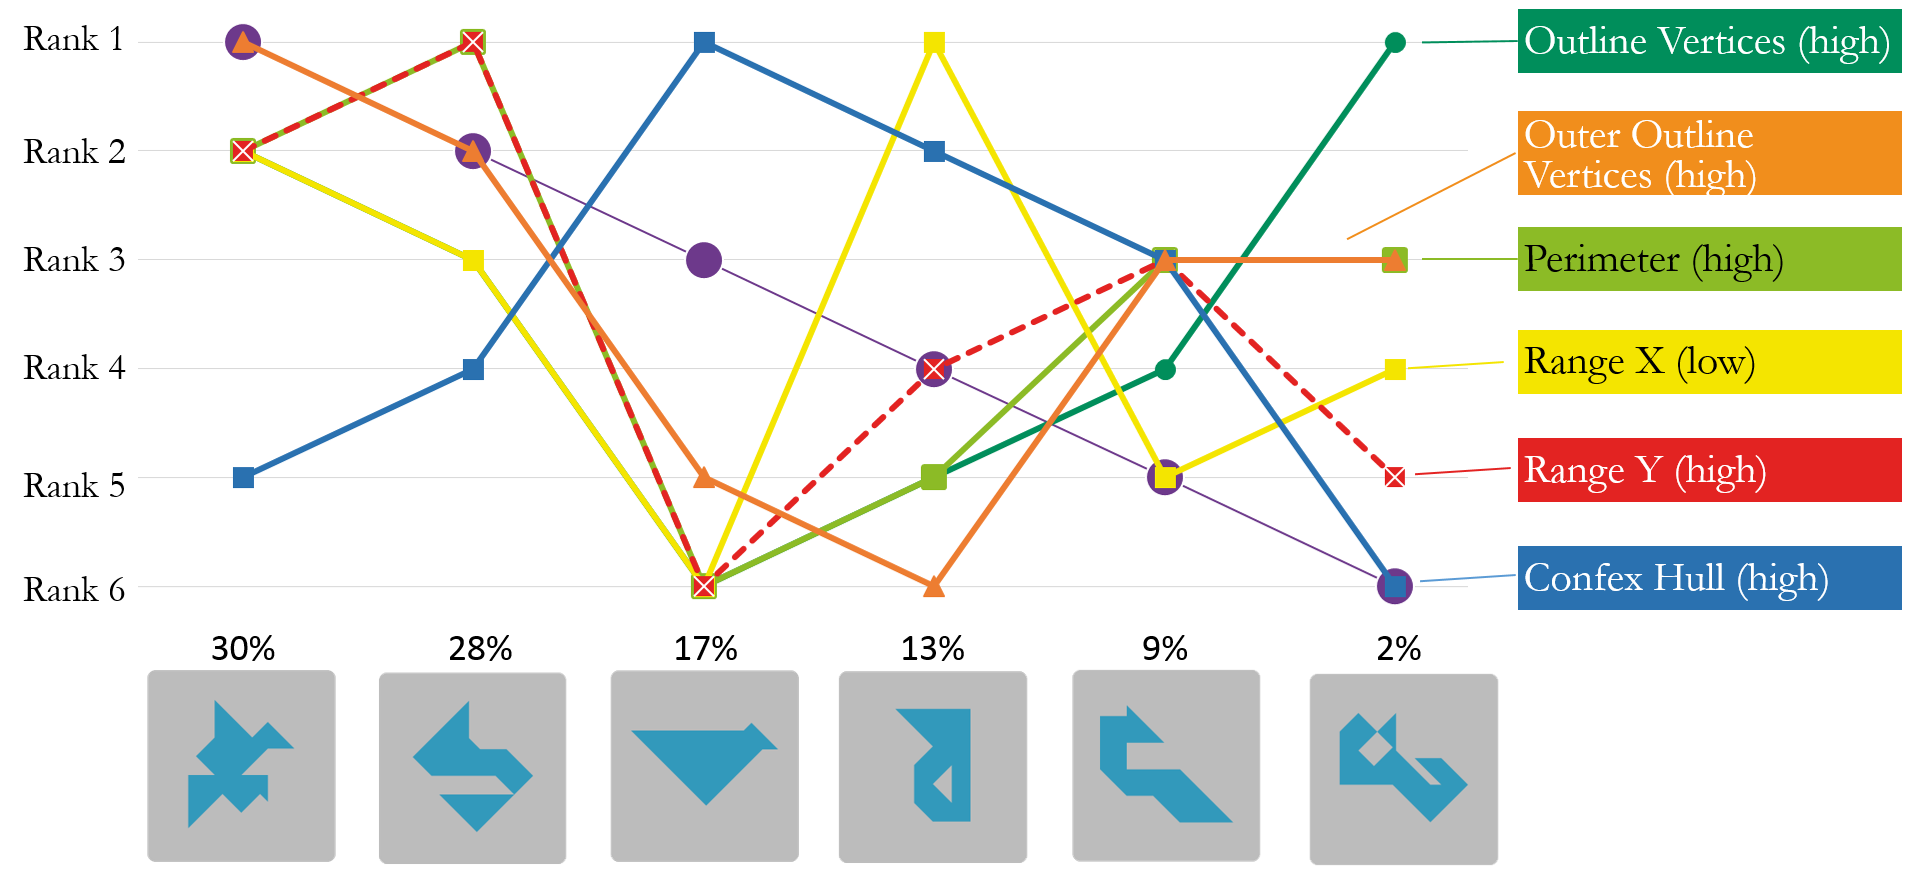
\includegraphics[width=0.95\textwidth]{figures/diagram.png}
  \caption{}  
  \label{result}
\end{figure}

Out of 1000 tangrams
with properties. 
compact
holes
just one hanging piece
small edges
First six were the same for all users
Overall .. took part. 